\documentclass[class=jsarticle, crop=false, dvipdfmx, fleqn]{standalone}
%% preamble for Numerical-structure-analysis report

\input{/Users/User/Documents/Project/TeX/preamble/mypreamble}

%% titles
\title{先端データ解析論 レポート}
\author{37-196360 \quad 森田涼介}


%% setting for listings
\newtcbinputlisting[auto counter]{\reportlisting}[3][]{%
	listing file = {#3},
	listing options = {language=python, style=tcblatex, numbers=left, numberstyle=\tiny},
	listing only,
	breakable,
	toprule at break = 0mm,
	bottomrule at break = 0mm,
	left = 6mm,
	sharp corners,
	drop shadow,
	title = Listings \thetcbcounter : \texttt{#2},
	label = #1,
	}



%% title format
\usepackage{titlesec}
\titleformat{\section}{\LARGE}{宿題\thesection}{0zw}{}
\newcommand{\sectionbreak}{\clearpage}
\titleformat{\subsection}{\Large}{\Alph{subsection})}{0zw}{}

\begin{document}
\section{}

直線モデル\(f_{\bm{\theta}} (x) = \theta_1 + \theta_2 x\)に対してテューキー回帰を行う。


\subsection*{理論}

微分可能で対称な損失\(\rho(r)\)に対して\(\tilde{r}\)で接する二次上界は,
(存在するなら)次式で与えられる。
\begin{equation}
    \tilde{\rho}(r) = \frac{\tilde{w}}{2} r + \mathrm{Const.}
        \qquad \qty(\tilde{w} = \frac{\rho^\prime (\tilde{r})}{\tilde{r}})
\end{equation}
これより,損失は次のように表される。
\begin{equation}
    J(\bm{\theta}) = \sum_{i=1}^{n} \rho\qty(f_{\mathrm{\bm{\theta}}} (\bm{x}_i) - y_i)
\end{equation}
また,\(J\)の上界は次式で表される。
\begin{align}
    \tilde{J}(\bm{\theta})
        & = \frac{1}{2} \sum_{i=1}^{n} \tilde{w}_i \qty(f_{\mathrm{\bm{\theta}}} (\bm{x}_i) - y_i) \\
        & = \frac{1}{2} (\bm{\Phi}\bm{\theta} - \bm{y})^\mathrm{T} \tilde{\bm{W}} (\bm{\Phi}\bm{\theta} - \bm{y})
\end{align}
ここで,
\begin{align}
	& \bm{\Phi} =
		\begin{bmatrix}
			\phi_1 (\bm{x}_1) & \cdots & \phi_b (\bm{x}_1) \\
			\vdots & \ddots & \vdots \\
			\phi_1 (\bm{x}_n) & \cdots & \phi_b (\bm{x}_n) \\
		\end{bmatrix} \\
	& \bm{y} =
		\begin{bmatrix}
			y_1 & \cdots & y_n
		\end{bmatrix}^\mathrm{T} \\
	& \tilde{\bm{W}} = \mathrm{diag}\qty{\tilde{w}_1,\ \cdots,\ \tilde{w}_n}
\end{align}
である。
これを最小にするパラメータは,
\(\bm{\Phi}^\mathrm{T}\tilde{\bm{W}}\bm{\Phi}\)の逆行列が存在することを仮定すると次式で与えられる。
\begin{equation}
    \hat{\bm{\theta}} = \qty(\bm{\Phi}^\mathrm{T}\tilde{\bm{W}}\bm{\Phi})^{-1} \bm{\Phi}^\mathrm{T} \tilde{\bm{W}}\bm{y}
    \label{eq:theta}
\end{equation}

テューキー損失は次式で表される。
\begin{equation}
    \rho(r) =
        \begin{cases}
            \frac{1}{6} \qty{1 - (1 - (r/\eta)^2)^3} & (|r| \le \eta) \\
            \frac{1}{6} & (|r| > \eta)
        \end{cases}
\end{equation}
これより,重みは次のように表される。
\begin{equation}
    \tilde{w} =
        \begin{cases}
            \qty(1 - \qty(\frac{r}{\eta})^2)^2 & (|r| \le \eta) \\
            0 & (|r| > \eta)
        \end{cases}
    \label{eq:w_turkey}
\end{equation}

以上より,以下の手順でパラメータを求めればよい。
\begin{enumerate}
    \item \(\bm{\theta}\)を適当に初期化する
    \item 式(\ref{eq:w_turkey})を用いて\(\tilde{\bm{W}}\)を計算する
    \item 式(\ref{eq:theta})を用いて\(\bm{\theta}\)を更新する
    \item 2,3を収束するまで繰り返す
\end{enumerate}



\subsection*{結果}

\(\eta = 0.5,\ 1.0,\ 1.5\)についての結果を示す。
表\ref{tab:result}に,\(\bm{\theta}\)の初期値と最終的な値,また収束時の損失を示した。
また,図\ref{fig:eta5}--\ref{fig:eta15}にプロットを示す。
なお,\(\bm{\theta}\)は\([0,\ 1)\)の一様分布で初期化した。
また,プログラムは\pageref{listing:assignment3}ページのListing \ref{listing:assignment3}に示した。

\begin{table}
    \centering
    \caption{結果}
    \begin{tabular}{cccccc}
        \(\eta\) & \(\theta_1\) (initial) & \(\theta_2\) (initial) & \(\theta_1\) & \(\theta_2\) & loss \\ \hline
        0.5 & 0.4427 & 0.9095 & 0.5170 & 1.024 & 3.759 \\
        1.0 & 0.8966 & 0.2608 & 0.1900 & 1.011 & 0.9676 \\
        1.5 & 0.9991 & 0.4859 & 0.2455 & 0.9955 & 0.5501
    \end{tabular}
    \label{tab:result}
\end{table}

\begin{figure}
	\centering
	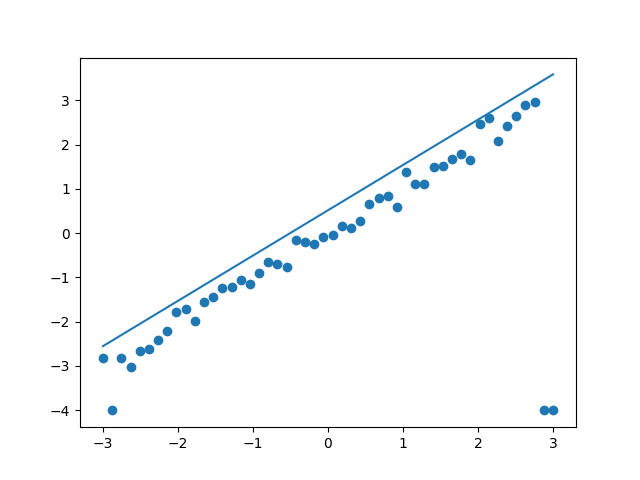
\includegraphics[clip, width=10cm]{../figures/assignment3_result_eta5}
	\caption{\(\eta = 0.5\)のときの実データと直線モデルのプロット}
	\label{fig:eta5}
\end{figure}

\begin{figure}
	\centering
	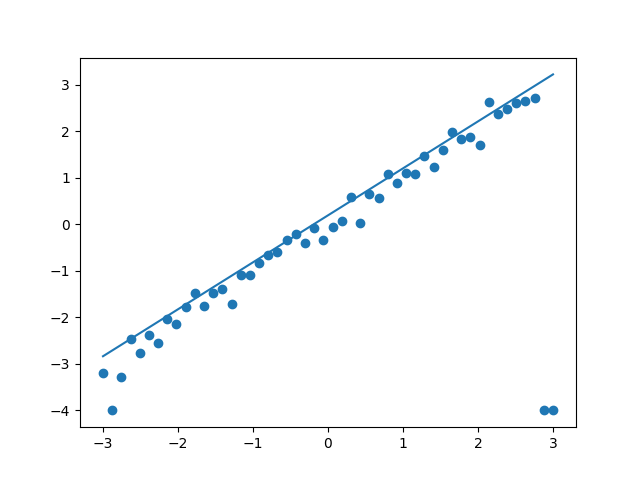
\includegraphics[clip, width=10cm]{../figures/assignment3_result_eta10}
	\caption{\(\eta = 1.0\)のときの実データと直線モデルのプロット}
	\label{fig:eta10}
\end{figure}

\begin{figure}
	\centering
	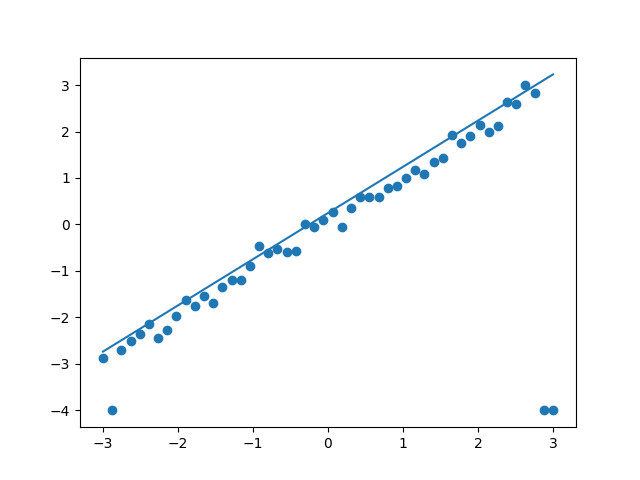
\includegraphics[clip, width=10cm]{../figures/assignment3_result_eta15}
	\caption{\(\eta = 1.5\)のときの実データと直線モデルのプロット}
	\label{fig:eta15}
\end{figure}


\end{document}
